\newpage
\section{Durchführung}
\label{sec:Durchführung}

\subsection{Versuchsaufbau}

Um die Wärmeleitfähigkeit von Aluminium, Edelstahl und den unterschiedlich
breiten Messingstäbe zu bestimmen werden diese gleichzeitig von einem
Peltierelement aufgeheizt und abgekühlt(siehe Abb. 1).
Anschließend wird die Temperatur erstens nah am Peltierelement und zweitens
im Abstand von $0,0303m$ gemessen und über einen Datenlogger ausgelesen.

Die Stäbe sind jeweils isoliert um die Wärmemenge
die an die Umgebung abgegeben wird zu reduzieren.


Die Stäbe haben folgende Ausmaße:
\begin{table}[h]
  \centering
  \label{tab:maß}
  \begin{tabular}{ c c }
    \toprule
    $Materialien$ & $ Abmessungen[cm]$
    \\
    \midrule
    Aluminium & 9\times 1,2\times 0,4  \\
    Messing(dünn) & 9\times 0,7\times 0,4   \\
    Messing(dick) & 9\times 1,2\times 0,4 \\
    Edelstahl & 9\times 1,2\times 0,4\\
    %$Wasser$ & 0 & 0 & 0 \\
    \bottomrule
  \end{tabular}
  \caption{Abmessungen }
\end{table}



\begin{figure}[h]
  \centering
  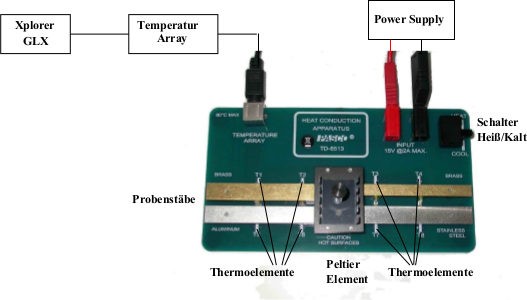
\includegraphics[width=\textwidth]{V204_Waermeleitung.png}
  \caption{Versuchsaufbau \cite{versuch}}
  \label{fig:waerm}
\end{figure}
\newpage
\subsection{statische Methode}
Bei der statischen Methode wird das Peltierelement mit der Spannung $U_P =5V$
und maximalen Strom versorgt und der Datenlogger trägt Werte im Abstand
 von $\increment t = 0,5 s$ auf bis die Messstelle  mit $T_7$ des Edelstahls
eine Temperatur von ca. \SI{45}{\degreeCelsius} erreicht. Danach werden die
Thermoelemente gekühlt und die Messwerte $T_1, T_4, T_5$ und $T_8$
des Datenloggers übertragen.

\subsection{dynamische Methode}
Die an das Peltierelement angelegte Spannung entspricht dieses mal $U_P = 8V$
und der Strom ist erneut maximal. Der Abstand mit dem die Temperaturen
gemessen werden wird auf $\increment t = 2s$ erhöht.
Sobald die Thermoelemente alle unter \SI{30}{\degreeCelsius} liegen wird
mit dem periodischen Heizen begonnen um die Wärmeleitfähigkeit anhand
einer Temperaturwelle zu bestimmen. Die Periode beträgt 80s bzw. es wird
40s geheizt und dann für 40s gekühlt. Dies wird für 10 Perioden wiederholt.
Anschließend werden die Thermoelemente erneut gekühlt und die Messwerte
$T_1$ und $T_2$ übertragen.

Nachdem die Thermoelemente wieder bei ungefähr \SI{30}{\degreeCelsius}
liegen wird eine zweite dynamische Messung durchgeführt. Dieses Mal wird
die Periode auf 200s erhöht und es sollen so viele Perioden durchlaufen
werden bis die Temperatur eines Thermoelements über \SI{80}{\degreeCelsius}
liegt. Zuletzt werden die Stäbe wieder auf Kühlung gestellt und die letzten
Werte $T_7$ und $T_8$ ausgelesen.
